%
% fp.tex
%
% (c) 2021 Prof Dr Andreas Müller, OST Ostschweizer Fachhochschule
%
\bgroup
\def\feld#1#2#3{
	\node at ({#1},{5-#2}) {$#3$};
}
\def\geld#1#2#3{
	\node at ({#1},{6-#2}) {$#3$};
}
\def\rot#1#2{
	\fill[color=red!20] ({#1-0.5},{5-#2-0.5}) rectangle ({#1+0.5},{5-#2+0.5});
}
\definecolor{darkgreen}{rgb}{0,0.6,0}
\def\gruen#1#2{
	\fill[color=darkgreen!20] ({#1-0.5},{6-#2-0.5}) rectangle ({#1+0.5},{6-#2+0.5});
}
\def\inverse#1#2{
	\node at (9,{6-#1}) {$#1^{-1}=#2\mathstrut$};
}
\begin{frame}[t]
\frametitle{Galois-Körper}
\vspace{-20pt}
\begin{columns}[t,onlytextwidth]
\begin{column}{0.48\textwidth}
\begin{block}{Restklassenring$\mathstrut$}
$\mathbb{Z}/n\mathbb{Z}
=\{ \llbracket r\rrbracket\;|\; 0\le r < n \} \mathstrut$
ist ein Ring
\end{block}
\uncover<2->{%
\begin{block}{Nullteiler}
Falls $n=n_1n_2$, dann sind $\llbracket n_1\rrbracket$ und
$\llbracket n_2\rrbracket$ Nullteiler in $\mathbb{Z}/n\mathbb{Z}$:
\[
\llbracket n_1\rrbracket
\llbracket n_2\rrbracket
=
\llbracket n_1n_2 \rrbracket
=
\llbracket n\rrbracket
=
\llbracket 0 \rrbracket
\]
\end{block}}
\end{column}
\begin{column}{0.48\textwidth}
\uncover<5->{%
\begin{block}{Galois-Körper $\mathbb{F}_p\mathstrut$}
$\mathbb{F}_p = \mathbb{Z}/p\mathbb{Z}\mathstrut$
\end{block}}
\uncover<4->{%
\begin{block}{$n$ prim}
Für $n=p$ prim ist $\mathbb{Z}/n\mathbb{Z}$ nullteilerfrei
\medskip

\uncover<5->{
$\Rightarrow \quad \mathbb{F}_p$ ist ein Körper
}
\end{block}}
\end{column}
\end{columns}
\vspace{-20pt}
\begin{center}
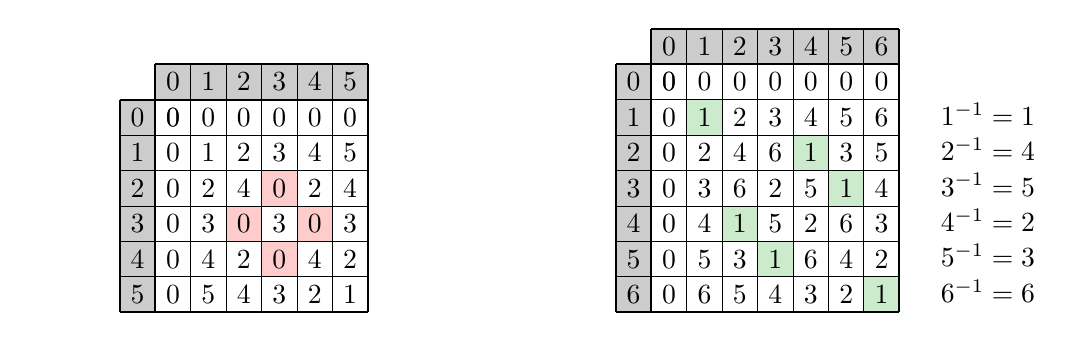
\begin{tikzpicture}[>=latex,thick,scale=0.45]
\fill[color=white] (-12,0) circle[radius=0.1];
\fill[color=white] (12,0) circle[radius=0.1];
\uncover<3->{
\begin{scope}[xshift=-8cm]
\rot{2}{3}
\rot{4}{3}
\rot{3}{2}
\rot{3}{4}
\fill[color=gray!40] (-0.5,5.5) rectangle (5.5,6.5);
\fill[color=gray!40] (-1.5,-0.5) rectangle (-0.5,5.5);
\foreach \x in {-0.5,5.5}{
	\draw (\x,-0.5) -- (\x,6.5);
}
\foreach \x in {0.5,...,4.5}{
	\draw[line width=0.3pt] (\x,-0.5) -- (\x,6.5);
}
\foreach \y in {0.5,...,5.5}{
	\draw[line width=0.3pt] (-1.5,\y) -- (5.5,\y);
}
\foreach \y in {-0.5,5.5}{
	\draw (-1.5,\y) -- (5.5,\y);
}
\draw (-1.5,-0.5) -- (-1.5,5.5);
\draw (-0.5,6.5) -- (5.5,6.5);
\foreach \x in {0,...,5}{
	\node at (\x,6) {$\x$};
	\node at (-1,{5-\x}) {$\x$};
}
\foreach \x in {0,...,5}{
	\feld{\x}{0}{0}
	\feld{0}{\x}{0}
}
\foreach \x in {2,...,5}{
	\feld{\x}{1}{\x}
	\feld{1}{\x}{\x}
}
\feld{1}{1}{1}
\feld{2}{2}{4}
\feld{2}{3}{0} \feld{3}{2}{0}
\feld{2}{4}{2} \feld{4}{2}{2}
\feld{2}{5}{4} \feld{5}{2}{4}
\feld{3}{3}{3}
\feld{4}{3}{0} \feld{3}{4}{0}
\feld{5}{3}{3} \feld{3}{5}{3}
\feld{4}{4}{4}
\feld{4}{5}{2} \feld{5}{4}{2}
\feld{5}{5}{1}
\end{scope}}
\uncover<6->{
\begin{scope}[xshift=6cm]
\uncover<7->{ \gruen{1}{1} }
\uncover<8->{ \gruen{4}{2} }
\uncover<9->{ \gruen{5}{3} }
\uncover<10->{ \gruen{2}{4} }
\uncover<11->{ \gruen{3}{5} }
\uncover<12->{ \gruen{6}{6} }
\fill[color=gray!40] (-0.5,6.5) rectangle (6.5,7.5);
\fill[color=gray!40] (-1.5,-0.5) rectangle (-0.5,6.5);
\foreach \x in {-0.5,6.5}{
	\draw (\x,-0.5) -- (\x,7.5);
}
\foreach \x in {0.5,...,5.5}{
	\draw[line width=0.3pt] (\x,-0.5) -- (\x,7.5);
}
\foreach \y in {0.5,...,6.5}{
	\draw[line width=0.3pt] (-1.5,\y) -- (6.5,\y);
}
\foreach \y in {-0.5,6.5}{
	\draw (-1.5,\y) -- (6.5,\y);
}
\draw (-1.5,-0.5) -- (-1.5,6.5);
\draw (-0.5,7.5) -- (6.5,7.5);
\foreach \x in {0,...,6}{
	\node at (\x,7) {$\x$};
	\node at (-1,{6-\x}) {$\x$};
}
\foreach \x in {0,...,6}{
	\geld{\x}{0}{0}
	\geld{0}{\x}{0}
}
\foreach \x in {2,...,6}{
	\geld{\x}{1}{\x}
	\geld{1}{\x}{\x}
}
\geld{1}{1}{1}
\geld{2}{2}{4}
\geld{2}{3}{6} \geld{3}{2}{6}
\geld{2}{4}{1} \geld{4}{2}{1}
\geld{2}{5}{3} \geld{5}{2}{3}
\geld{2}{6}{5} \geld{6}{2}{5}
\geld{3}{3}{2}
\geld{4}{3}{5} \geld{3}{4}{5}
\geld{5}{3}{1} \geld{3}{5}{1}
\geld{6}{3}{4} \geld{3}{6}{4}
\geld{4}{4}{2}
\geld{5}{4}{6} \geld{4}{5}{6}
\geld{6}{4}{3} \geld{4}{6}{3}
\geld{5}{5}{4}
\geld{6}{5}{2} \geld{5}{6}{2}
\geld{6}{6}{1}
\uncover<7->{ \inverse{1}{1} }
\uncover<8->{ \inverse{2}{4} }
\uncover<9->{ \inverse{3}{5} }
\uncover<10->{ \inverse{4}{2} }
\uncover<11->{ \inverse{5}{3} }
\uncover<12->{ \inverse{6}{6} }
\end{scope}}
\end{tikzpicture}
\end{center}
\end{frame}
\egroup
